%% (Master) Thesis template
% Template version used: v1.4
%
% Largely adapted from Adrian Nievergelt's template for the ADPS
% (lecture notes) project.


%% We use the memoir class because it offers a many easy to use features.
\documentclass[11pt,a4paper,table]{memoir}  %% TODO: Maybe ,titlepage needs to be added?

%% Packages
%% ========

%% LaTeX Font encoding -- DO NOT CHANGE
\usepackage[OT1]{fontenc}

%% Babel provides support for languages.  'english' uses British
%% English hyphenation and text snippets like "Figure" and
%% "Theorem". Use the option 'ngerman' if your document is in German.
%% Use 'american' for American English.  Note that if you change this,
%% the next LaTeX run may show spurious errors.  Simply run it again.
%% If they persist, remove the .aux file and try again.
\usepackage[english]{babel}

%% Input encoding 'utf8'. In some cases you might need 'utf8x' for
%% extra symbols. Not all editors, especially on Windows, are UTF-8
%% capable, so you may want to use 'latin1' instead.
\usepackage[utf8]{inputenc}

%% This changes default fonts for both text and math mode to use Herman Zapfs
%% excellent Palatino font.  Do not change this.
%\usepackage[sc]{mathpazo}

%% The AMS-LaTeX extensions for mathematical typesetting.  Do not
%% remove.
\usepackage{amsmath,amssymb,amsfonts,mathrsfs}

%% NTheorem is a reimplementation of the AMS Theorem package. This
%% will allow us to typeset theorems like examples, proofs and
%% similar.  Do not remove.
%% NOTE: Must be loaded AFTER amsmath, or the \qed placement will
%% break
\usepackage[amsmath,thmmarks]{ntheorem}

%% LaTeX' own graphics handling
\usepackage{graphicx}

%% We unfortunately need this for the Rules chapter.  Remove it
%% afterwards; or at least NEVER use its underlining features.
\usepackage{soul}

%% This allows you to add .pdf files. It is used to add the
%% declaration of originality.
\usepackage{pdfpages}

%% Some more packages that you may want to use.  Have a look at the
%% file, and consult the package docs for each.
%% See the TeXed file for more explanations

%% [OPT] Multi-rowed cells in tabulars
%\usepackage{multirow}

%% [REC] Intelligent cross reference package. This allows for nice
%% combined references that include the reference and a hint to where
%% to look for it.
\usepackage{varioref}

%% [OPT] Easily changeable quotes with \enquote{Text}
%\usepackage[german=swiss]{csquotes}

%% [REC] Format dates and time depending on locale
\let\ordinal\relax %% prevent warning
\usepackage{datetime}

%% [OPT] Provides a \cancel{} command to stroke through mathematics.
%\usepackage{cancel}

%% [NEED] This allows for additional typesetting tools in mathmode.
%% See its excellent documentation.
\usepackage{mathtools}

%% [NEED] Conditional commands
\usepackage{ifthen}

%% [OPT] Manual large braces or other delimiters.
%\usepackage{bigdelim, bigstrut}

%% [REC] Alternate vector arrows. Use the command \vv{} to get scaled
%% vector arrows.
\usepackage[h]{esvect}

%% [NEED] Some extensions to tabulars and array environments.
\usepackage{array}

%% [OPT] Postscript support via pstricks graphics package. Very
%% diverse applications.
%\usepackage{pstricks,pst-all}

%% [?] This seems to allow us to define some additional counters.
%\usepackage{etex}

%% [ADV] XY-Pic to typeset some matrix-style graphics
%\usepackage[all]{xy}

%% [OPT] This is needed to generate an index at the end of the
%% document.
%\usepackage{makeidx}

%% [OPT] Fancy package for source code listings.  The template text
%% needs it for some LaTeX snippets; remove/adapt the \lstset when you
%% remove the template content.
\usepackage{listings}
% \lstset{language=TeX,basicstyle={\normalfont\ttfamily}}

%% [REC] Fancy character protrusion.  Must be loaded after all fonts.
%\usepackage[activate]{pdfcprot}

%% [REC] Nicer tables.  Read the excellent documentation.
\usepackage{booktabs}

%% [OPT] Package for adding TODOs.
\usepackage{todonotes}

%% [OPT] Package to define and use acronyms
\usepackage[nolist,nohyperlinks,smaller]{acronym}
 

%% Our layout configuration.  DO NOT CHANGE.
%% Memoir layout setup

%% NOTE: You are strongly advised not to change any of them unless you
%% know what you are doing.  These settings strongly interact in the
%% final look of the document.

% Dependencies
%\usepackage{ETHlogo}

% use helvetica as default font:
\usepackage[scaled]{helvet}
%\renewcommand\familydefault{\sfdefault} 

% Turn extra space before chapter headings off.
\setlength{\beforechapskip}{0pt}

\nonzeroparskip
\parindent=0pt
\defaultlists

% Chapter style redefinition
\makeatletter

\makepagestyle{headerWPageNr}% Create headerWPageNr style
\if@twoside
  \copypagestyle{headerWPageNr}{Ruled}
  \copypagestyle{chapter}{Ruled}
\else
  \copypagestyle{headerWPageNr}{ruled}
  \copypagestyle{chapter}{ruled}
\fi
% chapter pages have no header and center page number in footer:
\makeoddhead{chapter}{}{}{}
\makeevenhead{chapter}{}{}{}
\makeoddfoot{chapter}{}{\thepage}{}
\makeevenfoot{chapter}{}{\thepage}{}
\makeheadrule{chapter}{\textwidth}{0pt}

% all other pages have page number and chapter or section name in header without footer:
\makeoddhead{headerWPageNr}{\rightmark}{}{\thepage}
\makeevenhead{headerWPageNr}{\thepage}{}{\leftmark}
\makeoddfoot{headerWPageNr}{}{}{}
\makeevenfoot{headerWPageNr}{}{}{}
\pagestyle{headerWPageNr}% Set page style to headerWPageNr


\makechapterstyle{bianchimod}{%
  \copypagestyle{abstract}{empty}
  \chapterstyle{default}
  \renewcommand*{\chapnamefont}{\normalfont\Large\sffamily}
  \renewcommand*{\chapnumfont}{\normalfont\Large\sffamily}
  \renewcommand*{\printchaptername}{%
    \chapnamefont\centering\@chapapp}
  \renewcommand*{\printchapternum}{\chapnumfont {\thechapter}}
  \renewcommand*{\chaptitlefont}{\normalfont\huge\sffamily}
  \renewcommand*{\printchaptertitle}[1]{%
    \hrule\vskip\onelineskip \centering \chaptitlefont\textbf{\vphantom{gyM}##1}\par}
  \renewcommand*{\afterchaptertitle}{\vskip\onelineskip \hrule\vskip
    \afterchapskip}
  \renewcommand*{\printchapternonum}{%
    \vphantom{\chapnumfont {9}}\afterchapternum}}
  
\makechapterstyle{bianchimod2}{%
  \renewenvironment{abstract}{\chapter*{\abstractname}}{}
  \chapterstyle{default}
  \definecolor{ChapGrey}{rgb}{0.6,0.6,0.6}
  \newcommand{\LargeFont}{% Needs a ’stretchable’ font
  	\usefont{\encodingdefault}{\sfdefault}{b}{n}%
    \fontsize{100}{0}\selectfont\color{ChapGrey}}
  \renewcommand*{\chapnumfont}{\LargeFont}
  \renewcommand*{\printchaptername}{\raggedleft}
  \renewcommand*{\printchapternum}{\chapnumfont {\thechapter}}
  \renewcommand*{\chaptitlefont}{\normalfont\Huge\sffamily\color{black}}
  \renewcommand*{\printchaptertitle}[1]{%
    \raggedleft \chaptitlefont\textbf{\vphantom{gyM}##1}\par}}

% Use the newly defined style
\chapterstyle{bianchimod2}

\setsecheadstyle{\Large\bfseries\sffamily}
\setsubsecheadstyle{\large\bfseries\sffamily}
\setsubsubsecheadstyle{\bfseries\sffamily}
\setparaheadstyle{\normalsize\bfseries\sffamily}
\setsubparaheadstyle{\normalsize\itshape\sffamily}
\setsubparaindent{0pt}

% Set captions to a more separated style for clearness
\captionnamefont{\sffamily\bfseries\footnotesize}
\captiontitlefont{\sffamily\footnotesize}
\setlength{\intextsep}{16pt}
\setlength{\belowcaptionskip}{1pt}

% Set section and TOC numbering depth to subsection
\setsecnumdepth{subsection}
\settocdepth{subsection}

% definitions for titlepage
\def\@advisor{}
\newcommand{\advisor}[1]{\def\@advisor{#1}}
\def\@supervisor{}
\newcommand{\supervisor}[1]{\def\@supervisor{#1}}
\def\@group{}
\newcommand{\group}[1]{\def\@group{#1}}
\def\@institute{}
\newcommand{\institute}[1]{\def\@institute{#1}}
\def\@department{}
\newcommand{\department}[1]{\def\@department{#1}}
\def\@school{}
\newcommand{\school}[1]{\def\@school{#1}}
\def\@thesistype{}
\newcommand{\thesistype}[1]{\def\@thesistype{#1}}
\def\@email{}
\newcommand{\email}[1]{\def\@email{#1}}

%% Title page adjustments
% the following definition (either 0 or 1) controls the title page's layout:
\def\centeredtitlepage{0}
\if\centeredtitlepage1
	% default title page from cadmo template
	\newcommand{\maketitlepage}{
		\begin{titlingpage}
  			\calccentering{\unitlength}
  			\begin{adjustwidth*}{\unitlength-24pt}{-\unitlength-24pt}
    		\maketitle
  			\end{adjustwidth*}
		\end{titlingpage}
	}
	\pretitle{\vspace{0pt plus 0.7fill}\begin{center}\HUGE\sffamily\bfseries}
	\posttitle{\end{center}\par}
	\preauthor{\par\begin{center}\let\and\\\Large\sffamily}
	\postauthor{\end{center}}
	\predate{\par\begin{center}\Large\sffamily}
	\postdate{\end{center}}

	\renewcommand{\maketitlehooka}{\noindent\ETHlogo[2in]}

	\renewcommand{\maketitlehookb}{\vspace{1in}%
  		\par\begin{center}\Large\sffamily\@thesistype\end{center}}

	\renewcommand{\maketitlehookd}{%
  		\vfill\par
  			\begin{flushright}
    			\sffamily
    			Advisors: \@supervisor, \@advisor\par
    			\@department, \@school
  			\end{flushright}
	}

\else
	% alternative title page (right-aligned)
	\newcommand{\maketitlepage}{
		\begin{titlingpage}
			\titlestyleright
		\end{titlingpage}
	}
	\newcommand*\titlestyleright{
		\thispagestyle{empty}
		\begin{minipage}[c]{0.35\linewidth}
			\vspace{0pt}
			
\includegraphics[width=0.9\linewidth]{images/ost_logo_de_rgb-eps-converted-to}
		\end{minipage}
		%
		\begin{minipage}[c]{0.4\linewidth}
			\vspace{0pt}
			\-\
		\end{minipage}
		%
		\begin{minipage}[c]{0.25\linewidth}
			\vspace{0pt}
			    \hspace*{-1cm} 
			        
\includegraphics[width=1.3\linewidth]{images/onway_logo}
		\end{minipage}
		\vspace{2cm}
		\sffamily
		\vspace*{\stretch{6}}
		\begin{flushright}
		{\Huge\sffamily\bfseries\@title\par}
		\par\noindent\rule[-1ex]{\linewidth}{2pt}\par
		\vspace{0.5cm}
		\emph{\huge\sffamily\@thesistype}
		\vspace{2cm}\par
		{\LARGE\sffamily\bfseries Florian Baumgartner}\par
		{\sffamily\ \href{mailto:florian.baumgartner@ost.ch}{florian.baumgartner@ost.ch}}\par
		\vspace{0.5cm}
		{\LARGE\sffamily\bfseries Luca Jost}\par
		{\sffamily\ \href{mailto:luca.jost@ost.ch}{luca.jost@ost.ch}}\par
		\vspace{1cm}
    	{\large\textbf{Advisor}\par
    		\@advisor\par}
    	\vspace{0.5cm}
    	{\large\textbf{Examiner}\par
    		\@supervisor\par}
    	\vspace{1cm}
    	{\@institute\par
        	\@school\par}
    	\vspace{1cm}
    	{\normalsize\@date\par}
		\end{flushright}
		\vspace{\stretch{1}}
		\noindent
		\pagebreak 
    	\sffamily
    	\thispagestyle{empty} 
	}
\fi

%Change margins
\setlrmarginsandblock{3.5cm}{3cm}{*}
\setulmarginsandblock{3cm}{*}{1}
\checkandfixthelayout

\setlength{\droptitle}{-48pt}

\makeatother

% This defines how theorems should look. Best leave as is.
\theoremstyle{plain}
\setlength\theorempostskipamount{0pt}

%%% Local Variables:
%%% mode: latex
%%% TeX-master: "thesis"
%%% End:


%% Theorem environments.  You will have to adapt this for a German
%% thesis.
%% Theorem-like environments

%% This can be changed according to language. You can comment out the ones you
%% don't need.

\numberwithin{equation}{chapter}

%% German theorems
%\newtheorem{satz}{Satz}[chapter]
%\newtheorem{beispiel}[satz]{Beispiel}
%\newtheorem{bemerkung}[satz]{Bemerkung}
%\newtheorem{korrolar}[satz]{Korrolar}
%\newtheorem{definition}[satz]{Definition}
%\newtheorem{lemma}[satz]{Lemma}
%\newtheorem{proposition}[satz]{Proposition}

%% English variants
\newtheorem{theorem}{Theorem}[chapter]
\newtheorem{example}[theorem]{Example}
\newtheorem{remark}[theorem]{Remark}
\newtheorem{corollary}[theorem]{Corollary}
\newtheorem{definition}[theorem]{Definition}
\newtheorem{lemma}[theorem]{Lemma}
\newtheorem{proposition}[theorem]{Proposition}

%% Proof environment with a small square as a "qed" symbol
\theoremstyle{nonumberplain}
\theorembodyfont{\normalfont}
\theoremsymbol{\ensuremath{\square}}
\newtheorem{proof}{Proof}
%\newtheorem{beweis}{Beweis}


%% Helpful macros.
%% Custom commands
%% ===============

%% Special characters for number sets, e.g. real or complex numbers.
\newcommand{\C}{\mathbb{C}}
\newcommand{\K}{\mathbb{K}}
\newcommand{\N}{\mathbb{N}}
\newcommand{\Q}{\mathbb{Q}}
\newcommand{\R}{\mathbb{R}}
\newcommand{\Z}{\mathbb{Z}}
\newcommand{\X}{\mathbb{X}}

%% Fixed/scaling delimiter examples (see mathtools documentation)
\DeclarePairedDelimiter\abs{\lvert}{\rvert}
\DeclarePairedDelimiter\norm{\lVert}{\rVert}

%% Use the alternative epsilon per default and define the old one as \oldepsilon
\let\oldepsilon\epsilon
\renewcommand{\epsilon}{\ensuremath\varepsilon}

%% Also set the alternate phi as default.
\let\oldphi\phi
\renewcommand{\phi}{\ensuremath{\varphi}}


%% This allow the usage of dashed and dotted lines in tables
\usepackage{arydshln}
\usepackage{hhline}
\usepackage{lscape}
\usepackage{siunitx}

\usepackage{caption}
\usepackage{subcaption}
\DeclareCaptionFont{fcaption}{\footnotesize}
%\captionsetup{labelfont={sf, bf}, textfont=sf, font=fcaption}
%\captionsetup[sub]{font=fcaption,labelfont={sf}}


%% Make document internal hyperlinks wherever possible. (TOC, references)
%% This MUST be loaded after varioref, which is loaded in 'extrapackages'
%% above.  We just load it last to be safe.
\usepackage[linkcolor=black,colorlinks=false,citecolor=black,filecolor=black]{hyperref}
\usepackage[capitalize, noabbrev]{cleveref}

%% Document information
%% ====================

\title{Fleet Monitoring System}
\author{}
\email{}
\thesistype{Seminar Paper}
\advisor{Martin Willi}
\supervisor{Prof.\ Beat Stettler}
\group{}
\institute{Institute for Networked Solutions}
\department{Department of Computer Science}
\school{Eastern Switzerland University of Applied Sciences}
\date{December 2021}

\begin{document}

\frontmatter

%% Title page is autogenerated from document information above.  DO
%% NOT CHANGE.
\maketitlepage

%% The abstract of your thesis.  Edit the file as needed.
\begin{abstract}
Onway AG offers WLAN and network access control solutions and software development. Their main fields of business are solutions for Network Access Control (NAC) as well as communication access for public transport. They are known for developing specialized industrial IoT applications. Onway AG is interested in providing an elegant solution for public transport fleets (e.g. buses) to gather low-level vehicle data and transmit them to a cloud-based system. This information can then be used to monitor the state of the vehicle and inform about possible issues in real time.

\todo[inline]{Add more blabla, maybe copy stuff from abstract tool?}

\end{abstract}


%% Temporary!
\subsubsection{General TODOs}
\todo[inline]{Luca, Add licensing block to all firmware code files}
\todo[inline]{Florian, Add licensing block to all python code files}
\todo[inline]{Florian, Create image of SD-Card from raspy and backup data on GitHub}
\todo[inline]{Florian, Update and finalize project schedule}
\todo[inline]{Luca, Create Test Reports}
\todo[inline]{Florian, List GitHub Repositories Links in Appendix}

%\clearpage

%% reset acronym usage:
\acresetall

%% TOC with the proper setup, do not change.
\cleartorecto
\tableofcontents
\mainmatter
\renewcommand{\thefigure}{\thechapter.\arabic{figure}}

%% acronyms used in this thesis:
\chapter*{Acronyms}
\begin{acronym}
\acro{WLAN}{Wireless LAN}
\acro{DCF}{Distributed Coordination Function}
\acro{AP}{Access Point}
\acro{IP}{Internet Protocol}
\acro{TCP}{Transmission Control Protocol}
\acro{UDP}{User Datagram Protocol}
\end{acronym}


%% Your real content!
%%\input{sections/1_task}
% Some commands used in this file
\newcommand{\package}{\emph}

\chapter{Introduction}
\section{Background}
Managing a large fleet of vehicles requires enormous effort. In order to minimize down time and offer seamless operation it is important to monitor the whole fleet on the road. Costs associated with operation, fuel, and maintenance can quickly mount. To ensure that fleet operations are as efficient and cost-friendly as possible, solutions are required to identify and eliminate any unnecessary expenditures. In general, fleet monitors can be used to improve efficiency, safety, and quality of fleet operations through the use of internet-connected sensors and software.

\newpage
\section{Product}

\bigskip
\begin{figure}[h!]
	\centering
	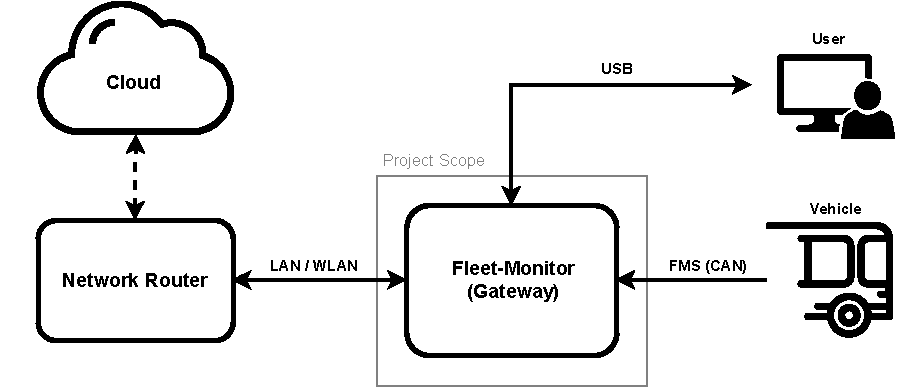
\includegraphics[width=\textwidth]{images/System_Overview}
	\vspace{-0.3cm}
	\caption{System Overview}
	\label{fig:system-overview}
\end{figure}

\section{Open Source}
From the beginning, it was decided that everything about the project would be released under an open source license. Both of us are huge supporters of open source and believe it will be the future of engineering. Building upon existing libraries and code under open source licences, allows us to accelerate the design process. Sometimes open source is considered an act of charity, but in our case, the benefits of using it outweigh any closed source processes. All documents and files of the project can be found on our GitHub page. A short description of all the repositories can be found in the Appendix \ref{Data Archive}.

\chapter{Requirements Specification and Project Schedule}

\theoremstyle{plain}
\theoremsymbol{}
\newtheorem{Rule}[theorem]{Rule}

\pagebreak
\section{Requirements Specification} \label{Requirements Specification}
\enlargethispage{2.5cm}
\begin{adjustwidth}{0.23cm}{0cm} \hfuzz=7.0pt
\makebox[\textwidth]{\frame{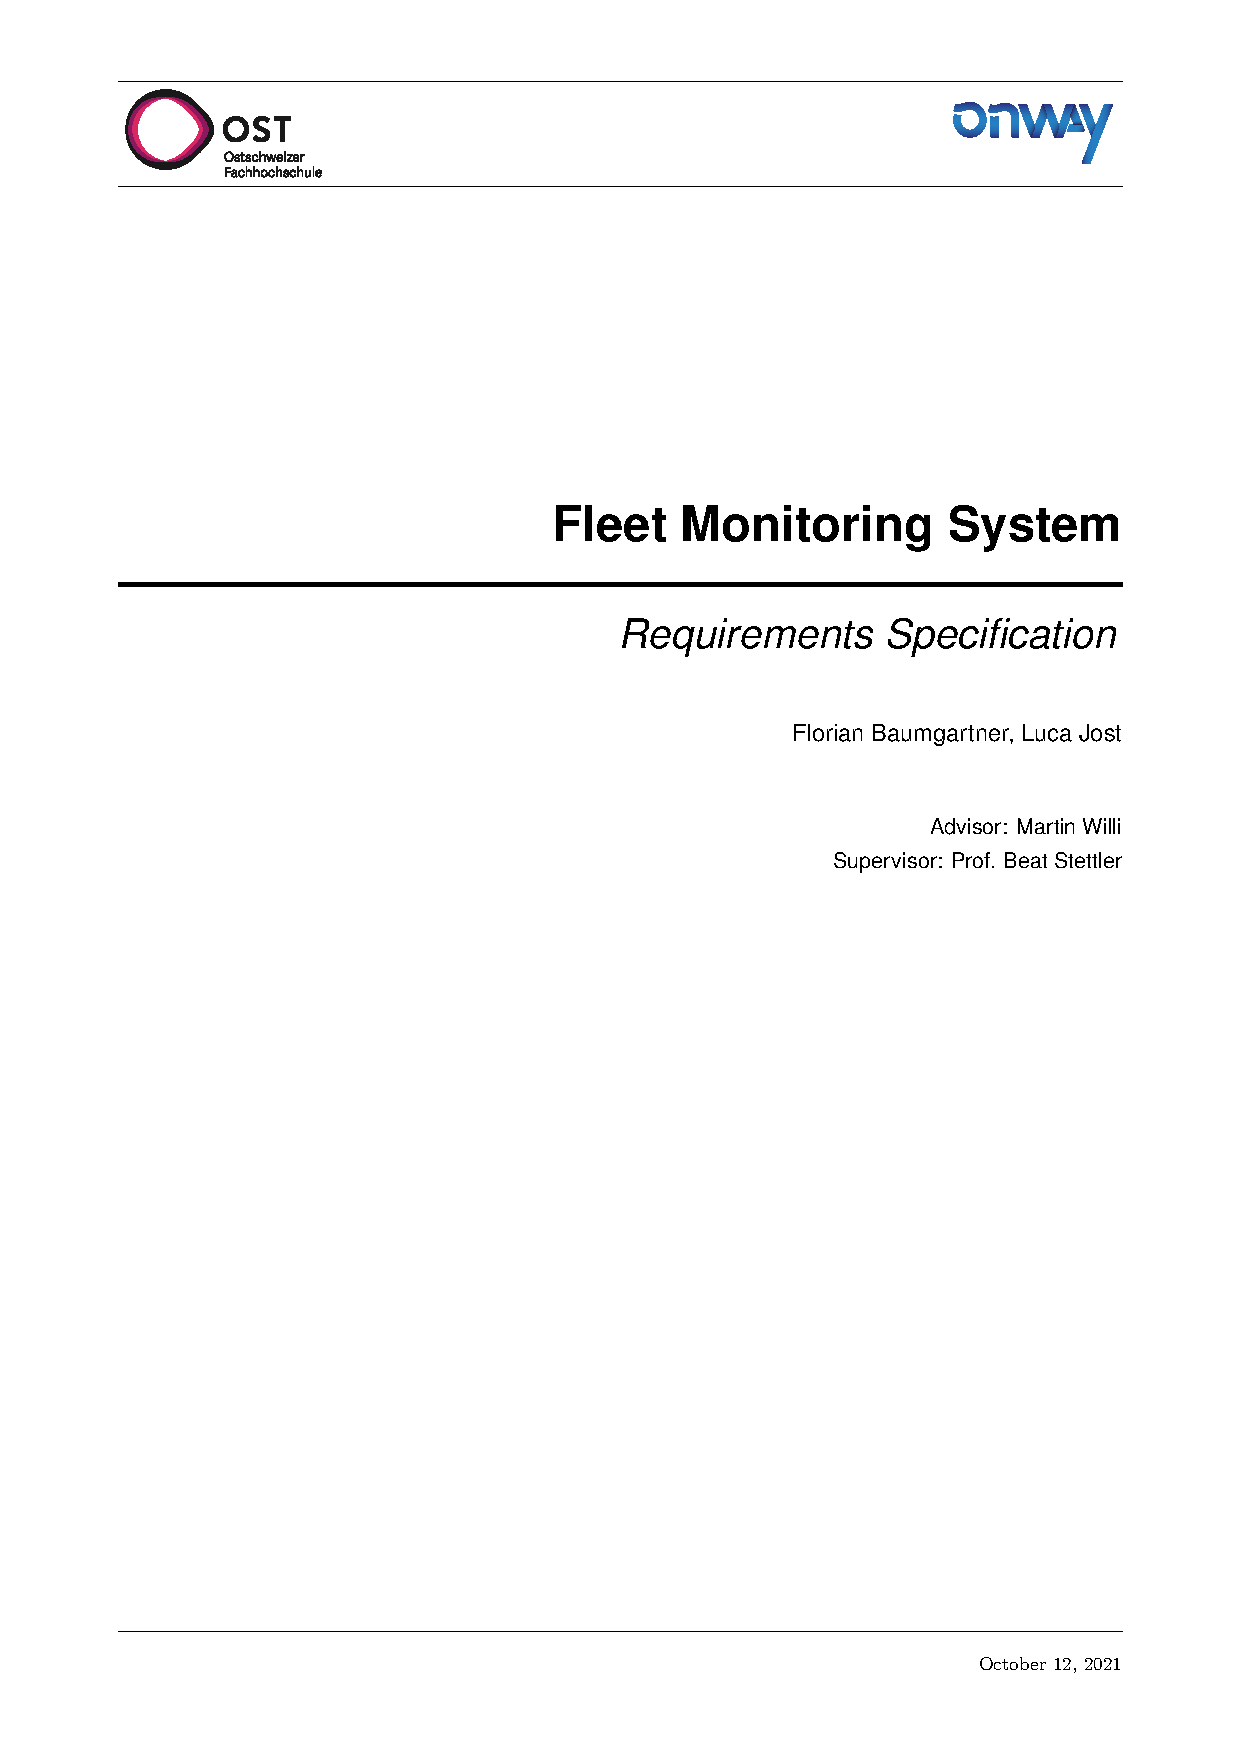
\includegraphics[width=17.3cm, page=1]{appendix/Requirements_Specification}}}
\end{adjustwidth}
\newpage

\begin{adjustwidth}{-0.23cm}{0cm} \hfuzz=7.0pt
\makebox[\textwidth]{\frame{\includegraphics[width=17.3cm, page=2]{appendix/Requirements_Specification}}}
\end{adjustwidth}
\newpage

\begin{adjustwidth}{0.23cm}{0cm} \hfuzz=7.0pt
\makebox[\textwidth]{\frame{\includegraphics[width=17.3cm, page=3]{appendix/Requirements_Specification}}}
\end{adjustwidth}
\newpage

\begin{adjustwidth}{-0.23cm}{0cm} \hfuzz=7.0pt
\makebox[\textwidth]{\frame{\includegraphics[width=17.3cm, page=4]{appendix/Requirements_Specification}}}
\end{adjustwidth}
\newpage

\begin{adjustwidth}{0.23cm}{0cm} \hfuzz=7.0pt
\makebox[\textwidth]{\frame{\includegraphics[width=17.3cm, page=5]{appendix/Requirements_Specification}}}
\end{adjustwidth}
\newpage

\begin{adjustwidth}{-0.23cm}{0cm} \hfuzz=7.0pt
\makebox[\textwidth]{\frame{\includegraphics[width=17.3cm, page=6]{appendix/Requirements_Specification}}}
\end{adjustwidth}
\newpage

\begin{adjustwidth}{0.23cm}{0cm} \hfuzz=7.0pt
\makebox[\textwidth]{\frame{\includegraphics[width=17.3cm, page=7]{appendix/Requirements_Specification}}}
\end{adjustwidth}
\newpage


\begin{landscape}
    \section{Project Schedule}
    \begin{figure}[h!]
    	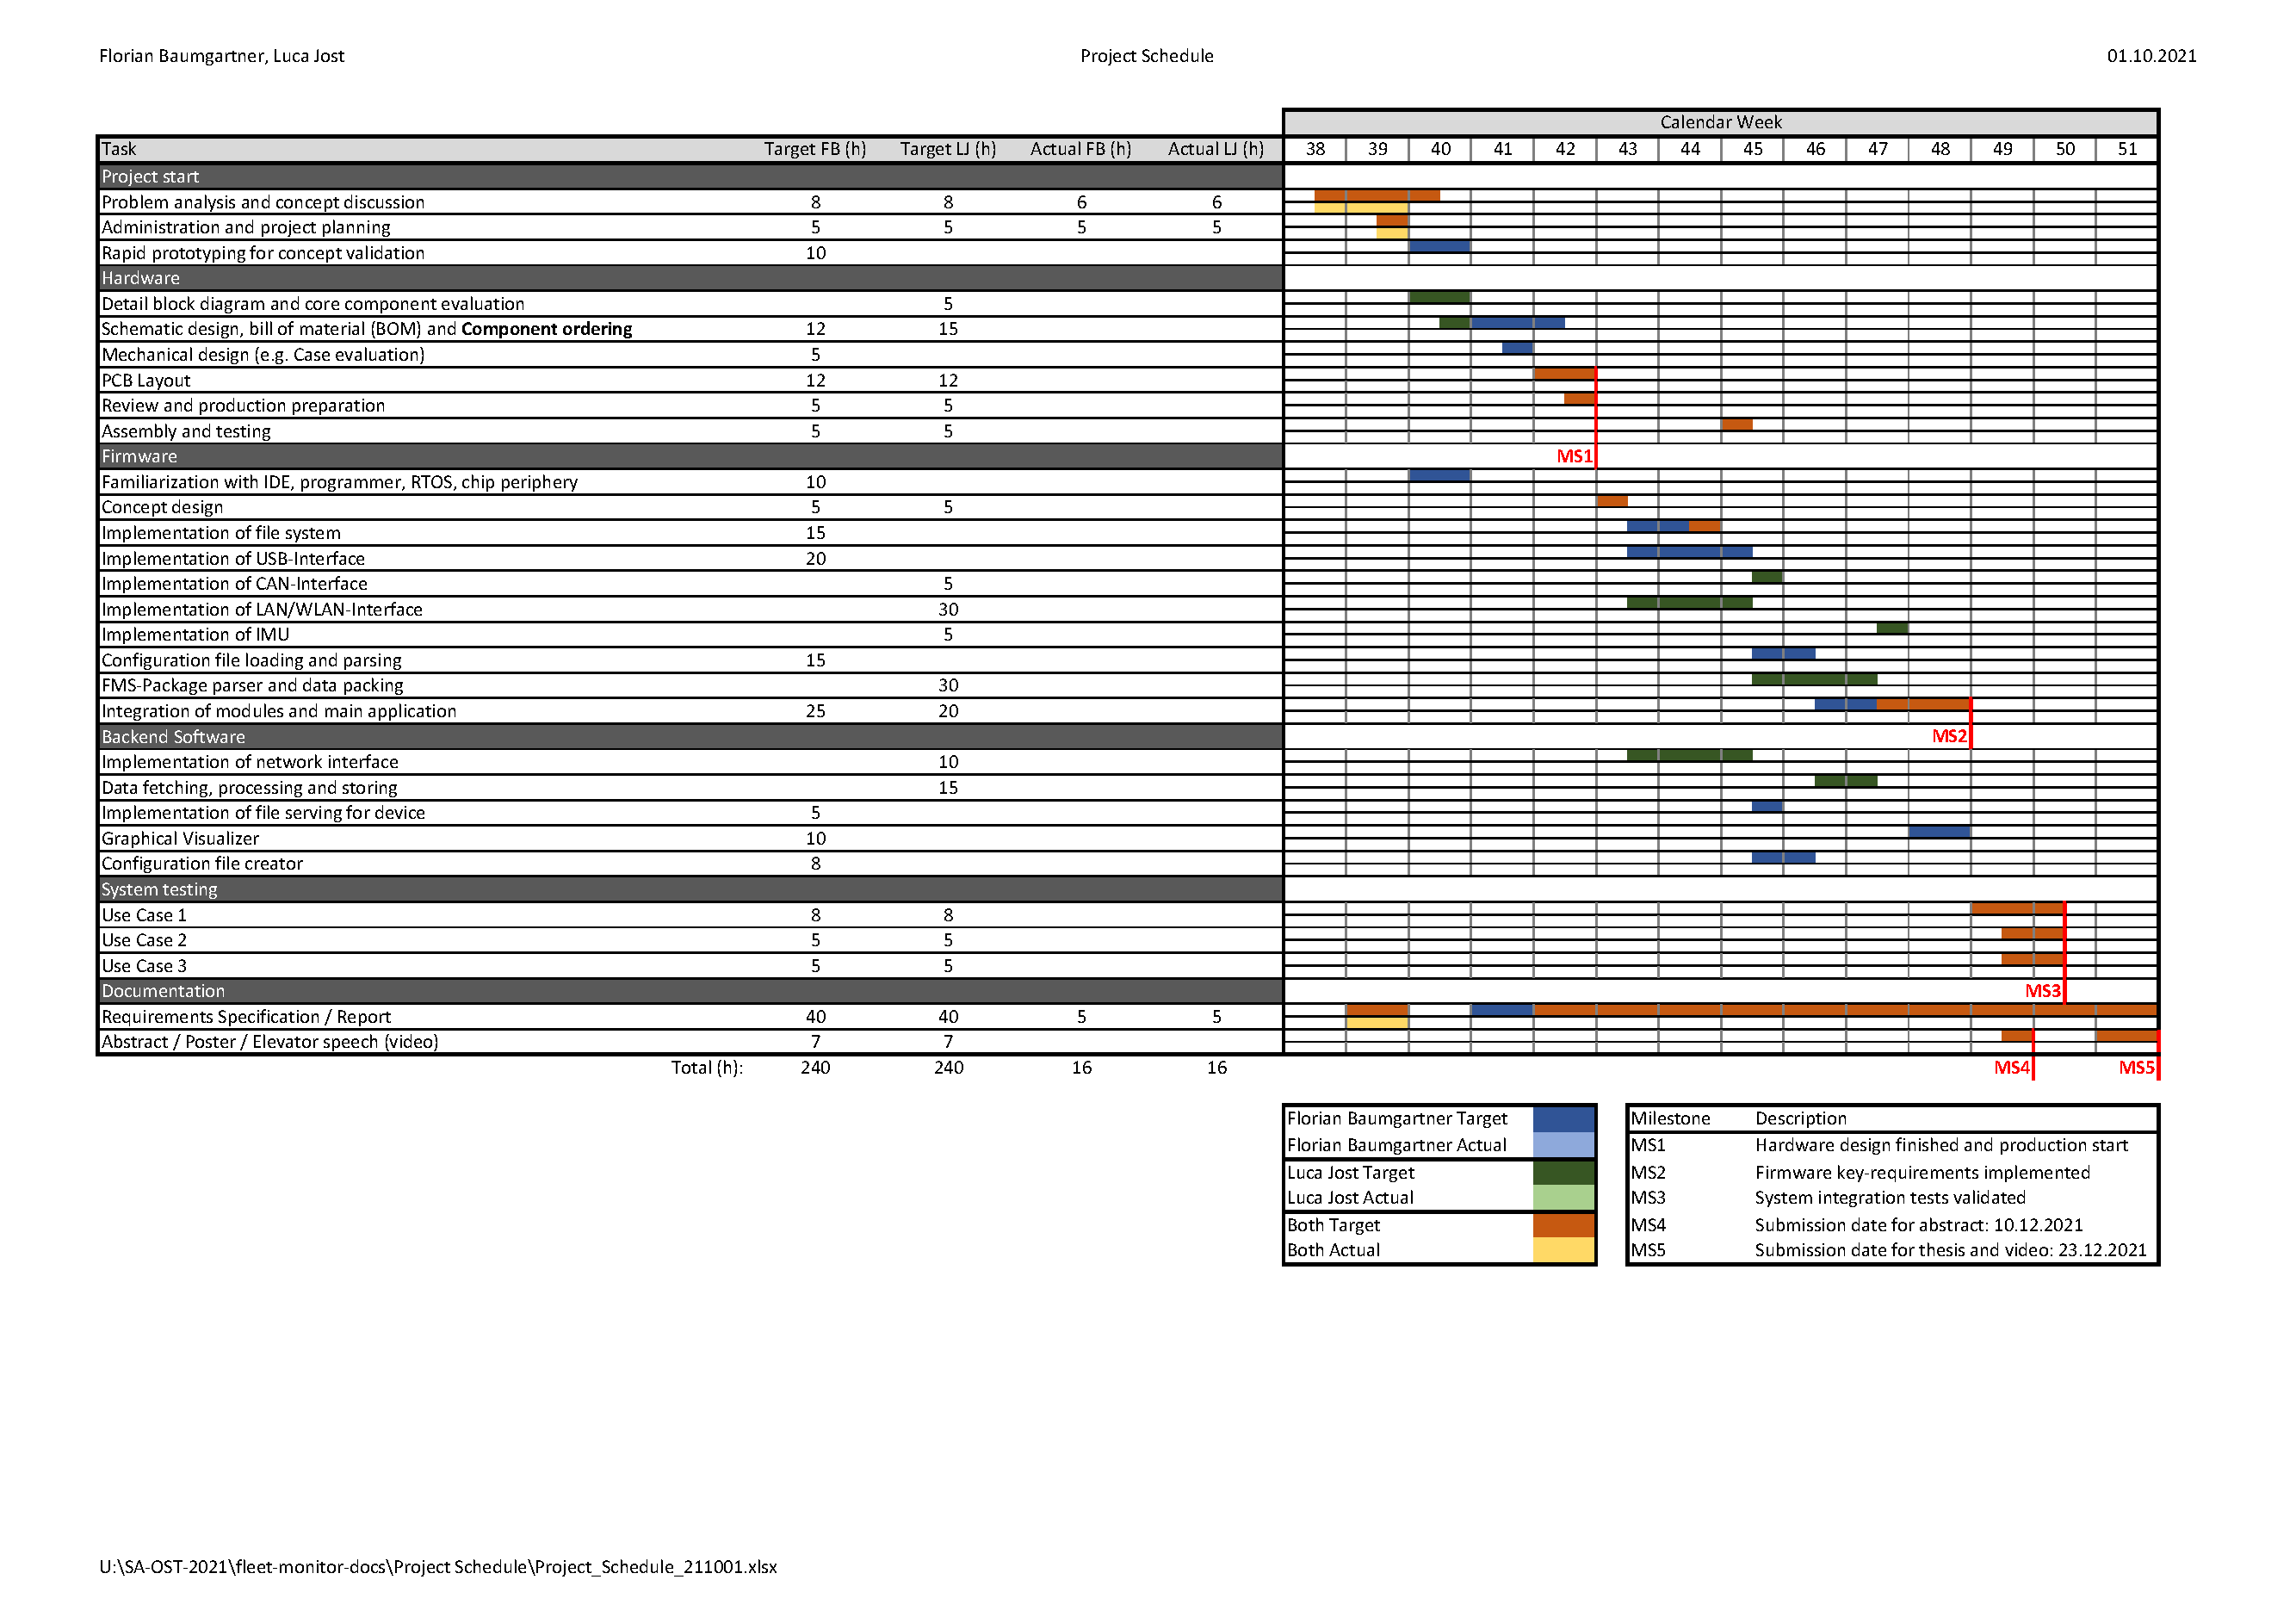
\includegraphics[height=13cm, trim=17mm 69mm 25mm 20mm, clip]{appendix/Project_Schedule_211001}
    	\bigskip
    	\caption{Project Schedule}
	    \vspace{-2cm}
	    \label{fig:project_schedule}
    \end{figure}
    \pagebreak

\end{landscape}
\chapter{System Overview}


\section{Punctuation}

\begin{Rule}
  Use opening (`) and closing (') quotation marks correctly.
\end{Rule}

In \LaTeX, the closing quotation mark is typed like a normal
apostrophe, while the opening quotation mark is typed using the French
\emph{accent grave} on your keyboard (the \emph{accent grave} is the
one going down, as in \emph{frère}).


%%% Local Variables:
%%% mode: latex
%%% TeX-master: "thesis"
%%% End:

\chapter{Hardware}

Dummy text. First use of an acronym: \ac{UDP}. Only short-hand of acronym is used when it reappears: \ac{UDP}.

\section{Example Section}

Dummy text.

\subsection{Example Subsection}

Dummy text.

\subsubsection{Example Subsubsection}

Dummy text.

\paragraph{Example Paragraph}

Dummy text.

\subparagraph{Example Subparagraph}

Dummy text. 

%%\input{sections/6_Measurements/6_measurements}
%%\input{sections/7_results}
%%\input{sections/8_summary_conclusion}

\appendix

\chapter{Dummy Appendix}

You can defer lengthy calculations that would otherwise only interrupt
the flow of your thesis to an appendix.


\backmatter

\bibliographystyle{plain}
\typeout{}
\bibliography{./sections/bibliography}

\end{document}